\documentclass{article}

\usepackage{fancyhdr}
\usepackage{extramarks}
\usepackage{amsmath}
\usepackage{amsthm}
\usepackage{amsfonts}
\usepackage{tikz}
\usepackage[plain]{algorithm}
\usepackage{algpseudocode}
\usepackage{listings} 
\usepackage{neuralnetwork}
\usepackage{subfigure}
\usetikzlibrary{automata,positioning}

\usepackage{color}

\definecolor{dkgreen}{rgb}{0,0.6,0}
\definecolor{gray}{rgb}{0.5,0.5,0.5}
\definecolor{mauve}{rgb}{0.58,0,0.82}

\lstset{frame=tb,
  language=Python,
  aboveskip=3mm,
  belowskip=3mm,
  showstringspaces=false,
  columns=flexible,
  basicstyle={\small\ttfamily},
  numbers=none,
  numberstyle=\tiny\color{gray},
  keywordstyle=\color{blue},
  commentstyle=\color{dkgreen},
  stringstyle=\color{mauve},
  breaklines=true,
  breakatwhitespace=true,
  tabsize=3
}
%
% Basic Document Settings
%

\topmargin=-0.45in
\evensidemargin=0in
\oddsidemargin=0in
\textwidth=6.5in
\textheight=9.0in
\headsep=0.25in

\linespread{1.1}

\pagestyle{fancy}
\lhead{\hmwkAuthorName}
\chead{\hmwkClass\: \hmwkTitle}
\rhead{\firstxmark}
\lfoot{\lastxmark}
\cfoot{\thepage}

\renewcommand\headrulewidth{0.4pt}
\renewcommand\footrulewidth{0.4pt}

\setlength\parindent{0pt}

%
% Create Problem Sections
%

\newcommand{\enterProblemHeader}[1]{
    \nobreak\extramarks{}{Task \arabic{#1} continued on next page\ldots}\nobreak{}
    \nobreak\extramarks{Task \arabic{#1} (continued)}{Problem \arabic{#1} continued on next page\ldots}\nobreak{}
}

\newcommand{\exitProblemHeader}[1]{
    \nobreak\extramarks{Task \arabic{#1} (continued)}{Problem \arabic{#1} continued on next page\ldots}\nobreak{}
    \stepcounter{#1}
    \nobreak\extramarks{Task \arabic{#1}}{}\nobreak{}
}

\setcounter{secnumdepth}{0}
\newcounter{partCounter}
\newcounter{homeworkProblemCounter}
\setcounter{homeworkProblemCounter}{1}
\nobreak\extramarks{Task \arabic{homeworkProblemCounter}}{}\nobreak{}

%
% Homework Problem Environment
%
% This environment takes an optional argument. When given, it will adjust the
% problem counter. This is useful for when the problems given for your
% assignment aren't sequential. See the last 3 problems of this template for an
% example.
%
\newenvironment{homeworkProblem}[1][-1]{
    \ifnum#1>0
        \setcounter{homeworkProblemCounter}{#1}
    \fi
    \section{Task \arabic{homeworkProblemCounter}}
    \setcounter{partCounter}{1}
    \enterProblemHeader{homeworkProblemCounter}
}{
    \exitProblemHeader{homeworkProblemCounter}
}

%
% Homework Details
%   - Title
%   - Due date
%   - Class
%   - Section/Time
%   - Instructor
%   - Author
%

\newcommand{\hmwkTitle}{Assignment\ \#3}
\newcommand{\hmwkDueDate}{March 10, 2019}
\newcommand{\hmwkClass}{CSCI964 Computational Intelligence}
\newcommand{\hmwkClassTime}{2.14}
\newcommand{\hmwkClassInstructor}{Zhifeng Wang}
\newcommand{\hmwkAuthorName}{\textbf{Mei Wangzhihui}}
\newcommand{\hmwkAuthorNum}{\textbf{2019124044}}
%
% Title Page
%

\title{
    \vspace{2in}
    \textmd{\textbf{\hmwkClass:\ \hmwkTitle}}\\
    % \normalsize\vspace{0.1in}\small{Due\ on\ \hmwkDueDate\ at 3:10pm}\\
    % \vspace{0.1in}\large{\textit{\hmwkClassInstructor\ \hmwkClassTime}}
    \vspace{3in}
}

\author{\hmwkAuthorName\ \hmwkAuthorNum}
\date{}

\renewcommand{\part}[1]{\textbf{\large Part \Alph{partCounter}}\stepcounter{partCounter}\\}

%
% Various Helper Commands
%

% Useful for algorithms
\newcommand{\alg}[1]{\textsc{\bfseries \footnotesize #1}}

% For derivatives
\newcommand{\deriv}[1]{\frac{\mathrm{d}}{\mathrm{d}x} (#1)}

% For partial derivatives
\newcommand{\pderiv}[2]{\frac{\partial}{\partial #1} (#2)}

% Integral dx
\newcommand{\dx}{\mathrm{d}x}

% Alias for the Solution section header
\newcommand{\solution}{\textbf{\large Solution}}

% Probability commands: Expectation, Variance, Covariance, Bias
\newcommand{\E}{\mathrm{E}}
\newcommand{\Var}{\mathrm{Var}}
\newcommand{\Cov}{\mathrm{Cov}}
\newcommand{\Bias}{\mathrm{Bias}}

\begin{document}

\maketitle

\pagebreak

\begin{homeworkProblem}
  \subsubsection{MNIST}
  The MNIST dataset is a handwritten dataset consisting 4 files: a training image set, a training label set, a test image set, a test label set; we can see that this is actually not an ordinary text file or image file, but a compressed file, download and unzip to get a binary file.
  \begin{itemize}
    \item train-images-idx3-ubyte.gz: training set images (9912422 bytes)
    \item train-labels-idx1-ubyte.gz: training set labels (28881 bytes)
    \item t10k-images-idx3-ubyte.gz: test set images (1648877 bytes)
    \item t10k-labels-idx1-ubyte.gz: test set labels (4542 bytes)
  \end{itemize}

  The MNIST dataset comes from the National Institute of Standards and Technology (NIST). M is the abbreviation of Modified. The training set is composed of numbers handwritten from 250 different people, of which 50\% are high school students and 50\% are from the Census Bureau staff. The test set is also the same proportion of handwritten digital data. Each picture is composed of 28x28 pixels, and each pixel is represented by a gray value. Here, the 28x28 pixels are expanded into a one-dimensional line vector (784 values per line). The picture label is one-hot code: 0-9.

  \begin{figure}[H]
    \centering
    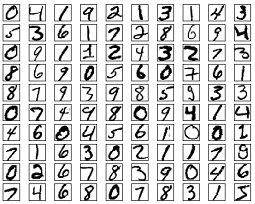
\includegraphics[width=.5\textwidth]{image/mnist1}
    \caption{The MNIST instances}
  \end{figure}
  \subsubsection{SOM}
  A Self-organizing Map is a data visualization technique developed by Professor Teuvo Kohonen in the early 1980's. Self-organizing maps are a class of unsupervised learning neural networks used for feature detection. They’re used to produce a low-dimension space of training samples. Therefore, they’re used for dimensionality reduction.
  \subsubsection{Model}

\end{homeworkProblem}

\begin{homeworkProblem}

\end{homeworkProblem}
\end{document}
